\documentclass[../mainfile.tex]{subfiles}
% Kopiert von kurbaniec :) 

\begin{document}
	\section{Berechnung des Differentialquotient}
	\subsection*{Beispiel:}
	Funktion für dieses Beispiel: $f(x) = x^{3} + x^{2} - x - 1$\\
	Steigung von $f(x)$ an der Stelle 2\\
	\\
	Differentialquotienten: $k = \lim\limits_{\triangle x \rightarrow 0}{\frac{\triangle f(x)}{\triangle x}} \Rightarrow \lim\limits_{\triangle x \rightarrow 0}{\frac{f(x+\triangle x)-f(x)}{\triangle x}}$
	\begin{figure}[h] 
		\centering
		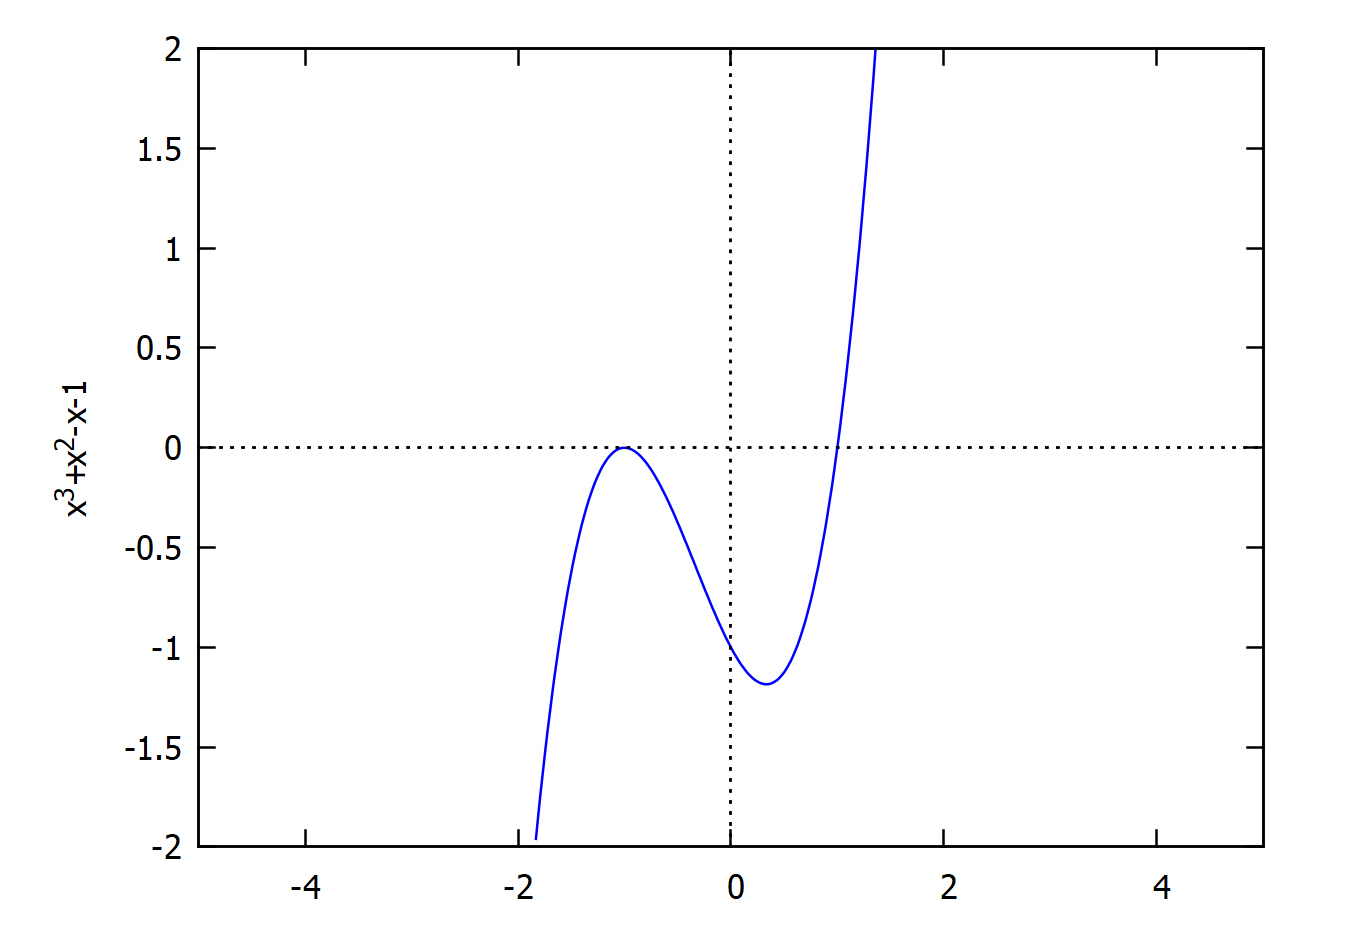
\includegraphics[width=8cm]{./swahl/img/graph2.jpg}
		\caption{Darstellung der Funktion}
	\end{figure}
	\\
	$\Rightarrow \lim\limits_{\triangle x \rightarrow 0}{\frac{(x+ \triangle x)^{3} + (x + \triangle x)^{2} - (x+ \triangle x) - 1 - (x^{3} + x^{2} - x - 1)}{\triangle x}}$\\
	$\Rightarrow \lim\limits_{\triangle x \rightarrow 0}{\frac{x^{3}+3x^{2}*\triangle x + 3x*(\triangle x)^{2} + (\triangle x)^{3}+ x^{2} + 2x*\triangle x + (\triangle x)^{2} - x - \triangle x -1 -x^{3} - x^{2} + x + 1 }{\triangle x}}$
	\\
	$\Rightarrow \lim\limits_{\triangle x \rightarrow 0}{\frac{3x^{2} * \triangle x + 3x * (\triangle x)^{2} + (\triangle x)^{3} + 2x * \triangle x + (\triangle x)^{2} - \triangle x}{\triangle x}}$
	\\
	$\Rightarrow \lim\limits_{\triangle x \rightarrow 0}{\frac{\triangle x * (3x^{2} + 3x * \triangle x + (\triangle x)^{2} + 2x+ \triangle x - 1) }{\triangle x}}$
	\\
	$\Rightarrow k = 3x^{2} + 2x - 1 \Rightarrow k$ an $2$ $\Rightarrow 12 + 4 - 1 = 15$
	\subsection*{Definition:}
	Eine Funktion heißt differenzierbar, wenn der Grenzwert $\lim\limits_{\triangle x \rightarrow 0}{\frac{\triangle f(x)}{\triangle x}}$ existiert.\\
	Dieser Grenzwert heißt erste Ableitung. $f'(x) \Rightarrow \frac{dy}{dx}$
	\subsection*{Bemerkung:}
	\begin{enumerate}
		\item[i)] $f'(x_{0})$ heißt erste Ableitung an der Stelle $x_{0}$
		\item[ii)] Eine differenzierbar Funktion ist dort im Intervall stetig. Das heißt eine stetige Funktion kann differenzierbar sein, muss es aber nicht.
	\end{enumerate}
\end{document}